\documentclass{beamer}
\usepackage{listings}
\lstset{
%language=C,
frame=single, 
breaklines=true,
columns=fullflexible
}
\usepackage{amsthm}
\usepackage{mathtools}
\usepackage{blkarray}
\usepackage{subcaption}
\usepackage{url}
\usepackage{tikz}
\usepackage{enumitem}
\usepackage{tkz-euclide} % loads  TikZ and tkz-base
%\usetkzobj{all}
\usetikzlibrary{calc,math}
\usepackage{float}
\newcommand{\myvec}[1]{\ensuremath{\begin{pmatrix}#1\end{pmatrix}}}
\providecommand{\brak}[1]{\ensuremath{\left(#1\right)}}
\newcommand\norm[1]{\left\lVert#1\right\rVert}
\renewcommand{\vec}[1]{\mathbf{#1}}
\usepackage[export]{adjustbox}
\usepackage[utf8]{inputenc}
\usepackage{amsmath}
\usepackage{physics}
\usepackage{tikz}
\usetikzlibrary{automata, positioning}
\usetheme{Boadilla}
\providecommand{\pr}[1]{\ensuremath{\Pr\left(#1\right)}}

\title{GATE ASSIGNMENT 1}
\author{ANANTHOJU PRANAV SAI - AI20BTECH11004}
\begin{document}
\begin{frame}
\titlepage
\end{frame}
\begin{frame}{Question}
    \begin{block}{GATE EC 2021 Q.39}
    The exponential Fourier series representation of a continuous-time periodic signal x(t) is defined as 
    \begin{align}
    x(t) = \sum_{k=-\infty}^{\infty}a_{k}e^{ik\omega_0t}
    \end{align}
    where $\omega_0$ is the fundamental angular frequency of $x(t)$ and the coefficients of the series are $a_k$. The following information is given about $x(t)$ and $a_k$.
    \begin{enumerate}[label=\Roman*]
    \item $x(t)$ is real and even, having a fundamental period of 6
    \item The average value of $x(t)$ is 2
    \item $a_k$ = $\begin{cases} 
                    k & 1\leq x\leq 3\\
                    0 & k>3
                  \end{cases}$
    \end{enumerate}
The average power of the signal $x(t)$ (rounded off to one decimal place) is
    \end{block}
\end{frame}
\begin{frame}{Parseval's Theorem}
\begin{theorem}[Parseval's power theorem]
If a exponential Fourier series representation of a continuous-time periodic signal x(t) is defined by 
\begin{align}
    x(t) = \sum_{n=-\infty}^{\infty}C_{n}e^{in\omega_0t}
\end{align}
where $C_n$ is given by
\begin{align}
    C_n = \frac{1}{T}\int_{0}^{T}x(t)e^{-jn\omega_0t}\,dt
\end{align}
then the average power of signal $x(t)$ is given by
\begin{align}
    \frac{1}{T}\int_{0}^{T}\lvert x(t)\rvert^2\,dt = \sum_{n=-\infty}^{\infty}\lvert C_n\rvert^2
\end{align}
\end{theorem}
\end{frame}
\begin{frame}
\begin{proof}
Given,
\begin{align}
    x(t) = \sum_{n=-\infty}^{\infty}C_{n}e^{in\omega_0t}     
\end{align}
Its complex conjugate can be written as
\begin{align}
    x(t)^* = \sum_{n=-\infty}^{\infty}C_{n}^*e^{-in\omega_0t}
\end{align}
Now we know that the average power of signal $x(t)$ is given by
\begin{align}
    P_{x(t)}&=\frac{1}{T}\int_{0}^{T}\lvert x(t)\rvert^2\,dt\\
    \implies P_{x(t)} &= \frac{1}{T}\int_{0}^{T}x(t)x(t)^*\,dt
\end{align}
\end{proof}
\end{frame}
\begin{frame}
\begin{block}{Proof Contd..}
\begin{align}
    \implies P_{x(t)} &= \frac{1}{T}\int_{0}^{T}x(t)\brak{\sum_{n=-\infty}^{\infty}C_{n}^*e^{-in\omega_0t}}\,dt\\
    \implies P_{x(t)} &= \sum_{n=-\infty}^{\infty}C_{n}^*\brak{\frac{1}{T}\int_{0}^{T}x(t)e^{-jn\omega_0t}\,dt}\\
    \implies P_{x(t)} &= \sum_{n=-\infty}^{\infty}C_{n}^*C_{n}\\
    \implies P_{x(t)} &= \sum_{n=-\infty}^{\infty}\lvert C_n\rvert^2
\end{align}
\end{block}
\end{frame}
\begin{frame}{Solution}
The given signal is defined as 
\begin{align}
    x(t) = \sum_{k=-\infty}^{\infty}a_{k}e^{ik\omega_0t}
\end{align}

where $a_k$ is Fourier Series Coefficient.
Given that the $x(t)$ is real and even. So the spectrum is also real and even.
$a_k$ = $\begin{cases} 
            k & 1\leq x\leq 3\\
            0 & k>3
        \end{cases}$\\  
% \begin{figure}[!h] 
%          \centering
%          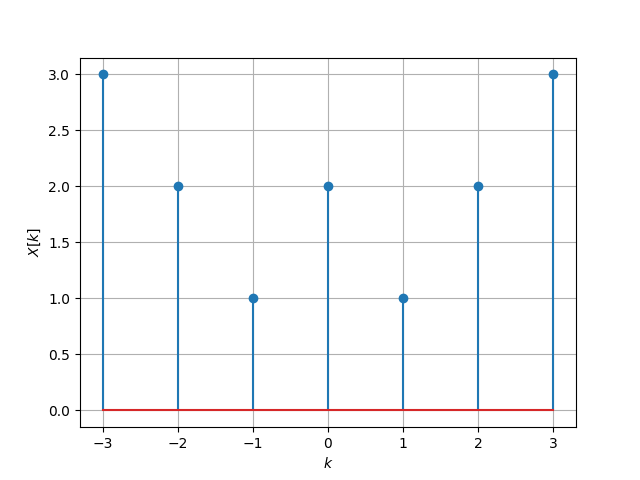
\includegraphics[width=\columnwidth]{plot.png}
%          \caption{Plot of the triangle}
%          \label{plot}
% \end{figure}
$\therefore$ Average power is :
\begin{align}
    \frac{1}{T}\int_{0}^{T}\lvert x(t)\rvert^2\,dt = \sum_{k=-3}^{3}\lvert a_k\rvert^2
\end{align}
\begin{align}
    P_{avg} &= 9+4+1+4+1+4+9\\
    P_{avg} &= 32
\end{align}
\end{frame}
\begin{frame}{Solution contd..}
\begin{figure}[!h]
         \centering
         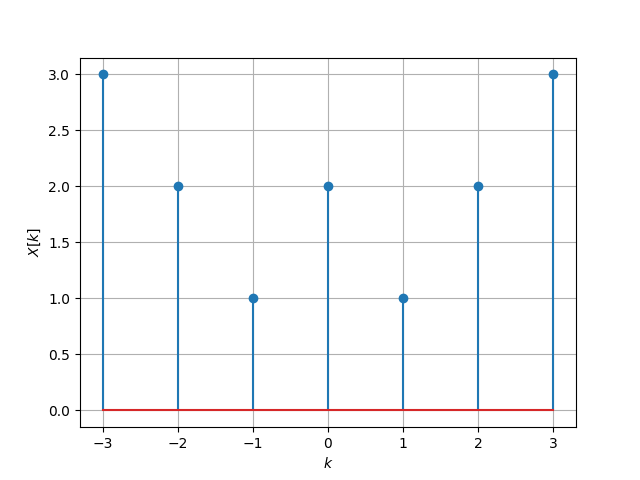
\includegraphics[width=10cm]{plot.png}
         \caption{Plot of $X[k]$}
         \label{plot}
\end{figure}
\end{frame}
\end{document}
